%Para este capítulo se usará la abreviatura "cam".
\chapter{Conexión por caminos}
\label{cam}

\begin{table}[H]
	\centering
	\begin{tabular}{c|c|c|c|c|}
		\cline{2-5}
		\multicolumn{1}{l|}{}                                                                                  & \multicolumn{1}{l|}{\textbf{Subespacios}}                             & \multicolumn{1}{l|}{\textbf{Cociente}} & \multicolumn{1}{l|}{\textbf{Producto}} & \multicolumn{1}{l|}{\textbf{Suma}} \\ \hline
		\multicolumn{1}{|c|}{\textbf{\begin{tabular}[c]{@{}c@{}}Conexo por\\ caminos\end{tabular}}}            & No                                                                    & Sí                                     & Sí                                     & No                                 \\ \hline
		\multicolumn{1}{|c|}{\textbf{\begin{tabular}[c]{@{}c@{}}Localmente conexo\\ por caminos\end{tabular}}} & \begin{tabular}[c]{@{}c@{}}Sí, en el caso \\ de abiertos\end{tabular} & Sí                                     & Sí                                     & Sí                                 \\ \hline
	\end{tabular}
	\caption{Tabla resumen de conexión por caminos}
	\label{Tabla_conexion_caminos}
\end{table}

\begin{figure}[h!]
	\centering
	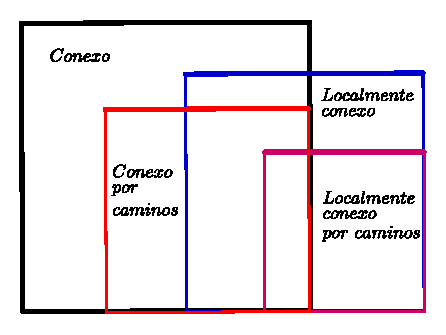
\includegraphics[scale = 1]{img/Comparacion_conexion}
	\caption{Ilustración de las relaciones entre las diferentes nociones de conexión.}
\end{figure}
